\documentclass{standalone}
\usepackage{tikz}

\usetikzlibrary{calc,math}


\begin{document}

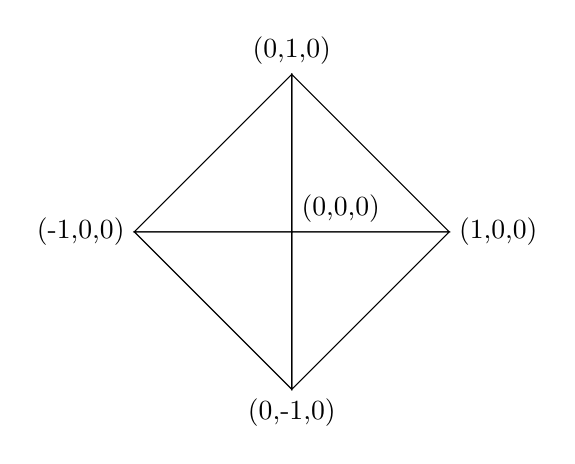
\begin{tikzpicture}
  \tikzmath{
    real \radius;
    \radius = 2;
  }
  \foreach[evaluate={\i + 90} as \j] \i in {0,90,...,270} {
    \draw (0,0) -- (\i:\radius) -- (\j:\radius) -- cycle;
  }
  \node[anchor=west] at (0:\radius) {(1,0,0)};
  \node[anchor=south] at (90:\radius) {(0,1,0)};
  \node[anchor=east] at (180:\radius) {(-1,0,0)};
  \node[anchor=north] at (270:\radius) {(0,-1,0)};
  \node[anchor=south west] at (0,0) {(0,0,0)};
\end{tikzpicture}

\end{document}